% !TeX root = Rapport.tex

\documentclass[12pt]{article}
\usepackage{lingmacros}
\usepackage{tree-dvips}
\usepackage[utf8]{inputenc}
\usepackage{fancyhdr}
\usepackage{listings}
\usepackage{xcolor}
\usepackage{geometry}
\usepackage{graphicx}
\usepackage{wrapfig}
\usepackage{amsmath}
\graphicspath{ {./img} }

 \geometry{
 a4paper,
 total={170mm,257mm},
 left=15mm,
 top=20mm,
 }


\definecolor{comment}{rgb}{0,0.45,0}
\definecolor{codegray}{rgb}{0.5,0.5,0.5}
\definecolor{codepurple}{rgb}{0.58,0,0.82}
\definecolor{backcolour}{rgb}{0.95,0.95,0.92}
\lstdefinestyle{CodeStyle}{
    backgroundcolor=\color{backcolour},   
    commentstyle=\color{comment},
    keywordstyle=\color{magenta},
    numberstyle=\tiny\color{codegray},
    stringstyle=\color{codepurple},
    basicstyle=\ttfamily\footnotesize,
    breakatwhitespace=false,         
    breaklines=true,                 
    captionpos=b,                    
    keepspaces=true,                 
    numbers=left,                    
    numbersep=5pt,                  
    showspaces=false,                
    showstringspaces=false,
    showtabs=false,                  
    tabsize=2
}
\lstset{style=CodeStyle}
\lstdefinelanguage{JavaScript}{
  keywords={typeof, new, true, false, catch, function, return, null, catch, switch, var, if, in, while, do, else, case, break},
  keywordstyle=\color{purple}\bfseries,
  ndkeywords={class, export, const, var, let, boolean, throw, implements, import, this, !!, !=, ===, ;},
  ndkeywordstyle=\color{blue}\bfseries,
  identifierstyle=\color{black},
  sensitive=false,
  comment=[l]{//},
  morecomment=[s]{/*}{*/},
  commentstyle=\color{comment}\ttfamily,
  stringstyle=\color{orange}\ttfamily,
  morestring=[b]',
  morestring=[b]"
}

%%%%%%% Document begin %%%%%%%%%%%
\begin{document}

\title{Dijkstra's Algoritme}
\author{Johannes Jørgensen\\ S2o}
\date{2021 Febuar}
\maketitle
\pagebreak
\tableofcontents
\pagebreak

%% Introduktion
\section{Introduktion}
Dijkstra's Algoritme er en kendt algoritmen indenfor pathfinding. Formål er at finde den korteste vej fra punkt a til punkt b. Dette er en større del af almindelige menneskers liv end man tænker. Hvad er den hurtigste vej til skole eller arbejde? Er det via motorvejen som måske har vejarbejde? Vil det så være hurtigere at tag vejen igennem byen? Disse spørgsmål kan man ofte få hurtigt svar på med ens GPS, som har implementeret diverse pathfinding algoritmer og er tilkoblet internettet med de seneste nyheder om vejarbejde, kø osv. 
\\Jeg vil med brug af Dijkstra's Algoritme finde sammenhængen mellem den matematiske del af rekursion som og et rekursion-kald i programmering.  

%% Teori
\section{Teori}

% Hvad er rekursion?
\subsection{Hvad er rekursion?}
Ordet rekursion er en betegnelse for noget som refererer til sig selv. Når noget refererer sig selv betyder det at noget behøver information eller data fra sit forrige jeg. Rekursion er oftest betegnet som en rekursionligning i matematik og en som en funktion der kalder sig selv i programmering. 

%Rekursion i Matematik
\subsection{Rekursion i Matematik}

%% Programmering
\subsection{Programmering}
% Rekursion i programmering
\subsubsection{Rekursion i programmering}
Rekursion i programmering er en funktion som har et rekursivts kald, alså funktion kalder sig selv. Dette kald kan være meget direkte som i eksempel 1 (Simpel rekursions funktion), eller indirekte hvor det ikke er lige så overskuligt at se et rekursivt kald.
\begin{lstlisting}[language=JavaScript, caption=Simpel rekursions funktion]
function fractorial(n) {        
  if (n == 1) return 1; 
  else return n*fractorial(n-1) 
} // if n = 4, then exprected output: 24
\end{lstlisting}
Funktionen i eksempel 1 indtag en værdi \textit{n} som parameter. Hvis denne parameteren \textit{n} er 1 stopper det rekursive kald (se linje 2.). Dette betyder også at dette eksempel har et meget direkte grænse hvor \textit{n} ikke kan komme under 1. Linje 3 beskriver så hvordan \textit{n} skal reagere hvis dens værdi ikke er 1. Hvis \textit{n} ikke er 1, men eksempelvis 3 skal den gange nuværende \textit{n} med forrige \textit{n}. I forrige \textit{n} af 3 er 2, derfor skal 2 ganges med dens forrige \textit{n} og således.
\[n(1) = 1 \Leftrightarrow 1\] 
\[n(2) = 2*1 \Leftrightarrow   2\]
\[n(3) = 3*2 \Leftrightarrow   6\]
\[n(4) = 4*6 \Leftrightarrow  \textbf{24}\]

% Varialber
\subsubsection{Variabler}
Et variabel er en pladsholder for et stykke data. Typisk set bruger man variabler i brug når man skal gemme et stykke data som man skal bruge forskellige steder i programmet. Disse variabler kan ændres under programmets køretid afhængig i hvordan variables data bliver manipuleret. Variablers data kan eventuelt ændres under programmets køretid, hvis man ønsker. Lidt mere teknisk indeholder et variable særlige set af bits eller af variablenes datatype. Et variable har en datatype som identificere hvilke slags data variabelt kan indeholde. Diverse programmeringssprog bruger dynamiske datatyper, hvor variabler kan indeholde forskellige datatyper. Her et en tabel med forskellige datatyper.
\begin{table}[ht]
  \centering
  \begin{tabular}{ |c|c|c|c| }
   \hline
   \textbf{Datatype} & \textbf{Skrivemåder} & \textbf{Eksempel på data} & \textbf{Kommentar} \\ 
   \hline
   Integer & int & \small{…-3, -2, -1, 0, 1, 2,... 1000} & \shortstack{Kun heltal\\ \footnotesize{(både negativ og positiv)}} \\
   \hline
   Floating Point & float & …, -3.25, -2.11,... 100,12  & \shortstack{Decimaltal\\ \footnotesize{(både negativ og positiv)}} \\ 
   \hline
   String & str eller text & \shortstack{"hello world”, \\ "This is a string"}  &  \shortstack{Et række af karakterer\\ oftest tekst.} \\ 
   \hline
   Array & [ data1,data2,… ] & int val = [-2,-1,0,1,5] & \shortstack{Indeholder en række data \\ under et navn} \\ 
   \hline
   Character & char & @, s, ¤, k…  & Kun et symbol \\ 
   \hline
   Boolean & bool & True (1) eller False (0)  & Enten sandt eller falsk \\ 
   \hline
   Constant & const & "Hello", -3, 22, [1, 2, 3] & \shortstack{Dynamisk datatype, \\ men konstant værdi} \\ 
   \hline
  \end{tabular}
\end{table}

%Objekter
\subsubsection{Objekter}
Et objekt er en abstrakt enhed med specifikke karakteriseringer og opførelse. Et objekt kan være et variable, datastruktur, en funktion eller en kombination alle dem alle. Et praktiskt eksempl på dette kan være en bil som objekt. En bil har specifikke karakteriseringer såsom hjul, farve, producent osv. En bil har også opførsel som at starte motoren, accelerere bilen m.m. 
\\Hvis vi tager samme praktiske eksempel på en bil som objekt, kan vi overføre det til kode med en “Klasse” som er en form for plan over alle klassens objekter
\begin{lstlisting}[language=Java, caption=Eksempel på et objekt]
  class Car { // Blueprint a car
   int model;
   int year;
   string color;
   
    void drive() { // objekt
      // Get the car to drive
    }

    void reverse() { // objekt
      // Get the car to reverse
    }
}
\end{lstlisting}
%Arrays
\subsubsection{Arrays}
Et array er en datastruktur, der indeholder en gruppe af elementer. Disse elementer er typisk alle af samme datatype, såsom et integer eller en string. Arrays bruges typisk set i computerprogrammer til at organisere data, så et relateret sæt værdier nemt kan sorteres eller søges.
\begin{lstlisting}[language=JavaScript, caption=Eksempel på et array]
// Array with constant values of datatype String
const cars = ["Audi", "Volvo", "BMW"];
cars[0] = "Audi" // Index 0 of array
\end{lstlisting}

% Løkker
\subsubsection{Løkker}
En løkke er et stykke kode som vil fortsætte med at køre indtil en given betingelse er opfyldt. der er to slags løkker, “while” - løkker og “for”-løkker. “While” løkker kører ind til betingelsen i parentesen bliver opfyldt. Mens “for” løkker lavet selv et variabel, som i det simpleste tilfælde vil tælle op eller ned fra og køre det antal gange ifølge betingelse. Løkker er meget brugbare siden det stopper en fra at skulle skrive mange linjer af den samme kode hvis man skal køre noget flere gange.
\begin{lstlisting}[language=JavaScript, caption=Eksempel på et for løkke]
for (let i = 0; i < 5; i++) {
  console.log(i);
} // exprected output: 0,1,2,3,4
\end{lstlisting}

% Betinget udførelse
\subsubsection{Betinget udførelse (if statement)}
Betinget udførelse eller “if statement”, er et stykke kode som checker om en betingelse opfyldt nogle specifikke kriterier. Hvis de betingelser bliver opfyldt vil koden inde i dette if statement blive kørt. Med et if statement kan man give den flere kriterier ved at lave en “else if” eller “else” statement efter den første stykke kode. “else if” er et til if statement med en betingelse før den bliver kørt, samtidig med at dette stykke kode kun bliver kørt hvis det første if statement ikke opfylder sin betingelse. Et “else” statement er bare et stykke kode som vil blive kørt hvis koden ikke opfyldte sin betingelse.
\begin{lstlisting}[language=JavaScript, caption=Eksempel på betinget udførelse]
let val = 5; 

if(val == 1){
  console.log("The value is now 1!");
}else console.log("The value is not 1"); // exprected execution of statement
\end{lstlisting}
\subsubsection{Dijkstra's algoritme}
Dijkstra’s algoritme består af Breadth-First Search Algorithm (BFS) med et lille twist. BFS er designet til at søge igennem et data tree eller en graf struktur. BFS algoritmen søger først alle “neighbors” til et givne “node” før den søge i naboernes “children”. Twistet i Dijkstra's algoritme er dog Dijkstra gøre brug af en prioriterings kø af “nodes”, for at prioritere hvilke naboer Dijkstra’s skal søge igennem først. 
\\“Node” indenfor programmering er datapunkter i et data tree eller en anden form for datastruktur. “Neighbors” eller naboer er nodes som har direkte kommunikation for den første node. “Children” er så tredje leds nodes til første node. 
\begin{figure}[h]\label{gennemgang af datatree}
  \centering
  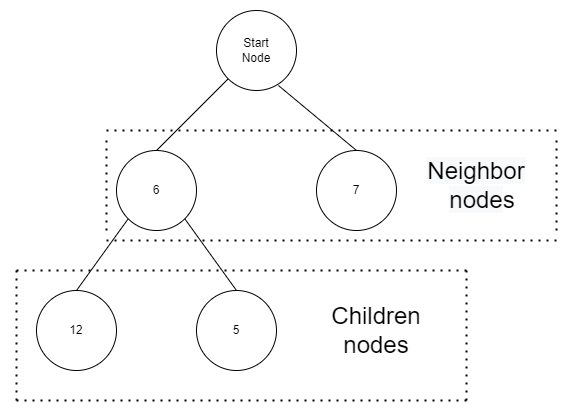
\includegraphics[width=0.80\textwidth]{img/nodeSetup.png}
  \caption{Illustration af et datatree med Nodes}
\end{figure}
\newpage
\begin{wrapfigure}{r}{0.40\textwidth} %this figure will be at the right 
  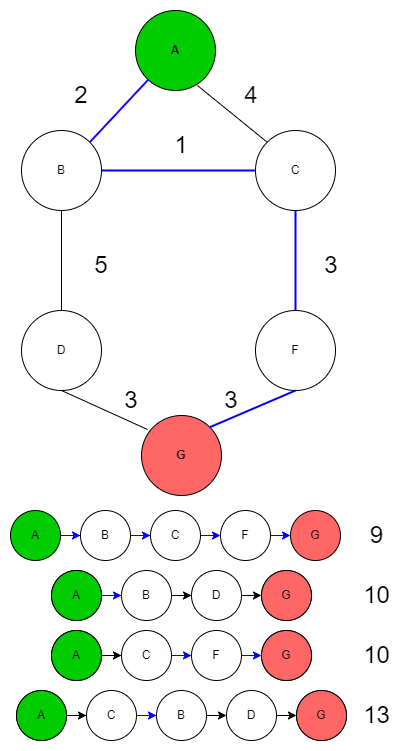
\includegraphics[width=0.4\textwidth, height=0.417\textheight]{img/AlgoViz.png}
  \caption{Eksempel på gennemgang af datatree af Dijkstra’s Algorithm}\label{eksempel af datatree}
  \centering
\end{wrapfigure}

Dijkstra’s algoritme er designet til at finde den korteste vej mellem 2 notes. Algorithmen søger og finder diverse veje med den korteste vej og beregner den korteste vej gennem hver node som ikke er søgt igennem. Derefter opdatere den nabo nodernes med den korteste vej imens den holder øje med hvilke nodes algoritmen allerede har søgt igennem. Vejen til hver node har en "vægt". En vægt betyder sværhedsgraden for at kommer til valgte node. Et praktisk eksempel på dette kunne være transport. En højere vægt værdi kan være på grund af eventuelt vejarbejde, kø osv. Figur \ref{eksempel af datatree} har også lignende vægte bare data raleterende.
\\Eksemplet her viser en datatree med følgende nodes $A,B,C,D,F,G$. Algoritmen skal finde den korteste vej fra node $A \rightarrow G$. Algorithmen vil først søge igennem nabo nodes til vores start node A. Vejen fra node $A \rightarrow B$ koster 2 og vejen fra $A \rightarrow C$ koster 4. Derfor indtil videre er den korteste vej B. Så søger algorithmen fra node $B \rightarrow C$ og D, vejen til C koster nu kun 3 ud fra forrige $A \rightarrow C$. Så søges vejen fra $C \rightarrow F$, og den er kortere end $B \rightarrow D$ som kostet 5. Til sidst søges den korteste vej fra $F \rightarrow G$ og $D \rightarrow G$, som vejen $F \rightarrow G$ er stadig den korteste vej. Dermed bliver den korteste vej $A \rightarrow B \rightarrow C \rightarrow F \rightarrow G$ med total vægtkost på 9. 

\subsubsection{Dijkstra’s Algorithm Pseudocode}
Nu når vi ved hvordan Dijkstra’s Algorithm virker skal vi prøve så oversætte det til kode.
Den bedste måde at generelt oversætte algoritmen kan vi lave en Pseudokode. En Pseudokode er en måde at skrive en algoritme eller en processen på en general programmerings måde uden at implementere direkte kode. Dette kan være hjælpe andre med generelt at forstå en algoritme kodemæssigt. 

\begin{lstlisting}[language=JavaScript, caption=Dijkstra’s Algorithm Pseudocode oversat til dansk]
function Dijkstra(G, S); // G = Graf, S = Source
  for hver V i G // V = vej
    afstand[V] = infinity // set alle veje til infinity
    forrige[V] = null
    hvis V != Start
      V += Q // Q = prioriterings queue
  afstand[S] // afstand fra node til node

  imens Q er tom
      U // U = min value fra Q
      for hver nabo V af U som stadig i Q
        midlertidigAfstand  // afstabd[U] + G.Sider[U, V]
        hvis midlertidigAfstand < afstand[V]
          afstand[V] // midlertidigAfstand
          forrige[V] // U

  return afstand[], forrige[]
\end{lstlisting}
\newpage
\section{Analyse}



% dijkstra algo
% \begin{lstlisting}[language=JavaScript, caption=Dijkstra's Algoritme]
% function dijkstra(
%   grid: CellProps[][],
%   startNode: CellProps,
%   finishNode: CellProps
% ) {
%   const visitedNodesInOrder = [];
%   startNode.distance = 0;
%   const unvisitedNodes = getAllCells(grid);
%   while (!!unvisitedNodes.length) {
%     sortCellsByDistance(unvisitedNodes);
%     const closestNode: CellProps | undefined = unvisitedNodes.shift();

%     if (closestNode != undefined) {
%       // If we encounter a wall, we skip it.
%       if (closestNode.isWall) continue;
%       // If the closest node is at a distance of infinity,
%       // we must be trapped and should therefore stop.
%       if (closestNode.distance === Infinity) return visitedNodesInOrder;
%       closestNode.isVisited = true;
%       visitedNodesInOrder.push(closestNode);
%       if (closestNode === finishNode) return visitedNodesInOrder;
%       updateUnvisitedNeighbors(closestNode, grid);
%     } else console.log("error, closestNode returned 0");
%   }
% }
% \end{lstlisting}

\end{document}